%% LyX 2.2.3 created this file.  For more info, see http://www.lyx.org/.
%% Do not edit unless you really know what you are doing.
\documentclass[ruled]{article}
\usepackage{courier}
\usepackage[T1]{fontenc}
\usepackage[latin9]{inputenc}
\usepackage[letterpaper]{geometry}
\geometry{verbose}
\usepackage{color}
\usepackage{algorithm2e}
\usepackage{amsmath}
\usepackage{amssymb}
\usepackage{graphicx}
\usepackage[unicode=true,
 bookmarks=false,
 breaklinks=false,pdfborder={0 0 1},backref=section,colorlinks=true]
 {hyperref}

\makeatletter

%%%%%%%%%%%%%%%%%%%%%%%%%%%%%% LyX specific LaTeX commands.
\providecommand{\LyX}{\texorpdfstring%
  {L\kern-.1667em\lower.25em\hbox{Y}\kern-.125emX\@}
  {LyX}}
%% A simple dot to overcome graphicx limitations
\newcommand{\lyxdot}{.}


\@ifundefined{date}{}{\date{}}
%%%%%%%%%%%%%%%%%%%%%%%%%%%%%% User specified LaTeX commands.
\definecolor{mygreen}{rgb}{0,0.6,0}
\definecolor{mygray}{rgb}{0.5,0.5,0.5}
\definecolor{mymauve}{rgb}{0.58,0,0.82}

\makeatother

\usepackage{listings}
\lstset{backgroundcolor={\color{white}},
basicstyle={\footnotesize\ttfamily},
breakatwhitespace=false,
breaklines=true,
captionpos=b,
commentstyle={\color{mygreen}},
deletekeywords={...},
escapeinside={\%*}{*)},
extendedchars=true,
frame=single,
keepspaces=true,
keywordstyle={\color{blue}},
language=Python,
morekeywords={*,...},
numbers=none,
numbersep=5pt,
numberstyle={\tiny\color{mygray}},
rulecolor={\color{black}},
showspaces=false,
showstringspaces=false,
showtabs=false,
stepnumber=1,
stringstyle={\color{mymauve}},
tabsize=2}
\begin{document}
\global\long\def\reals{\mathbf{R}}
 \global\long\def\integers{\mathbf{Z}}
 \global\long\def\naturals{\mathbf{N}}
 \global\long\def\rationals{\mathbf{Q}}
 \global\long\def\ca{\mathcal{A}}
 \global\long\def\cb{\mathcal{B}}
 \global\long\def\cc{\mathcal{C}}
 \global\long\def\cd{\mathcal{D}}
 \global\long\def\ce{\mathcal{E}}
 \global\long\def\cf{\mathcal{F}}
 \global\long\def\cg{\mathcal{G}}
 \global\long\def\ch{\mathcal{H}}
 \global\long\def\ci{\mathcal{I}}
 \global\long\def\cj{\mathcal{J}}
 \global\long\def\ck{\mathcal{K}}
 \global\long\def\cl{\mathcal{L}}
 \global\long\def\cm{\mathcal{M}}
 \global\long\def\cn{\mathcal{N}}
 \global\long\def\co{\mathcal{O}}
 \global\long\def\cp{\mathcal{P}}
 \global\long\def\cq{\mathcal{Q}}
 \global\long\def\calr{\mathcal{R}}
 \global\long\def\cs{\mathcal{S}}
 \global\long\def\ct{\mathcal{T}}
 \global\long\def\cu{\mathcal{U}}
 \global\long\def\cv{\mathcal{V}}
 \global\long\def\cw{\mathcal{W}}
 \global\long\def\cx{\mathcal{X}}
 \global\long\def\cy{\mathcal{Y}}
 \global\long\def\cz{\mathcal{Z}}
 \global\long\def\ind#1{1(#1)}
 \global\long\def\pr{\mathbb{P}}
 \global\long\def\predsp{\cy}
 \global\long\def\outsp{\cy}
 \global\long\def\prxy{P_{\cx\times\cy}}
 \global\long\def\prx{P_{\cx}}
 \global\long\def\prygivenx{P_{\cy\mid\cx}}
 \global\long\def\ex{\mathbb{E}}
 \global\long\def\var{\textrm{Var}}
 \global\long\def\cov{\textrm{Cov}}
 \global\long\def\sgn{\textrm{sgn}}
 \global\long\def\sign{\textrm{sign}}
 \global\long\def\kl{\textrm{KL}}
 \global\long\def\law{\mathcal{L}}
 \global\long\def\eps{\varepsilon}
 \global\long\def\as{\textrm{ a.s.}}
 \global\long\def\io{\textrm{ i.o.}}
 \global\long\def\ev{\textrm{ ev.}}
 \global\long\def\convd{\stackrel{d}{\to}}
 \global\long\def\eqd{\stackrel{d}{=}}
 \global\long\def\del{\nabla}
 \global\long\def\loss{\ell}
 \global\long\def\risk{R}
 \global\long\def\emprisk{\hat{R}_{\ell}}
 \global\long\def\lossfnl{L}
 \global\long\def\emplossfnl{\hat{L}}
 \global\long\def\empminimizer#1{\hat{#1}_{\ell}}
 \global\long\def\minimizer#1{#1_{*}}
 \global\long\def\etal{\textrm{et. al.}}
 \global\long\def\tr{\operatorname{tr}}
 \global\long\def\trace{\operatorname{trace}}
 \global\long\def\diag{\text{diag}}
 \global\long\def\rank{\text{rank}}
 \global\long\def\linspan{\text{span}}
 \global\long\def\proj{\text{Proj}}
 \global\long\def\argmax{\operatornamewithlimits{arg\, max}}
 \global\long\def\argmin{\operatornamewithlimits{arg\, min}}
 \global\long\def\bfx{\mathbf{x}}
 \global\long\def\bfy{\mathbf{y}}
 \global\long\def\bfl{\mathbf{\lambda}}
 \global\long\def\bfm{\mathbf{\mu}}
 \global\long\def\calL{\mathcal{L}}
 \global\long\def\vw{\boldsymbol{w}}
 \global\long\def\vx{\boldsymbol{x}}
 \global\long\def\vxi{\boldsymbol{\xi}}
 \global\long\def\valpha{\boldsymbol{\alpha}}
 \global\long\def\vbeta{\boldsymbol{\beta}}
 \global\long\def\vsigma{\boldsymbol{\sigma}}
 \global\long\def\vmu{\boldsymbol{\mu}}
 \global\long\def\vtheta{\boldsymbol{\theta}}
 \global\long\def\vd{\boldsymbol{d}}
 \global\long\def\vs{\boldsymbol{s}}
 \global\long\def\vt{\boldsymbol{t}}
 \global\long\def\vh{\boldsymbol{h}}
 \global\long\def\ve{\boldsymbol{e}}
 \global\long\def\vf{\boldsymbol{f}}
 \global\long\def\vg{\boldsymbol{g}}
 \global\long\def\vz{\boldsymbol{z}}
 \global\long\def\vk{\boldsymbol{k}}
 \global\long\def\va{\boldsymbol{a}}
 \global\long\def\vb{\boldsymbol{b}}
 \global\long\def\vv{\boldsymbol{v}}
 \global\long\def\vy{\boldsymbol{y}}
 \global\long\def\hil{\ch}
 \global\long\def\rkhs{\hil}
 

\title{Homework 2: Lasso Regression}

\maketitle
\textbf{Instructions}: Your answers to the questions below, including
plots and mathematical work, should be submitted as a single PDF file.
It's preferred that you write your answers using software that typesets
mathematics (e.g. \LaTeX{}, \LyX{}, or MathJax via iPython), though
scanning handwritten work is fine as well. You may find the \href{https://github.com/gpoore/minted}{minted}
package convenient for including source code in your \LaTeX{} document.
If you are using \LyX{}, then the \href{https://en.wikibooks.org/wiki/LaTeX/Source_Code_Listings}{listings}
package tends to work better.


\section{Introduction}

In this homework you will investigate regression with $\ell_{1}$
regularization, both implementation techniques and theoretical properties.
On the methods side, you'll work on coordinate descent (the ``shooting
algorithm''), homotopy methods, and {[}optionally{]} projected SGD.
On the theory side you'll derive the largest $\ell_{1}$ regularization
parameter you'll ever need to try, and optionally you'll derive the
explicit solution to the coordinate minimizers used in coordinate
descent, you'll investigate what happens with ridge and lasso regression
when you have two copies of the same feature, and you'll work out
the details of the classic picture that ``explains'' why $\ell_{1}$
regularization leads to sparsity.

\subsection{Data Set and Programming Problem Overview}

For the experiments, we are generating some artifical data using code
in the file \texttt{setup\_problem.py.} We are considering the regression
setting with the 1-dimensional input space $\reals$. An image of
the training data, along with the target function (i.e. the Bayes
prediction function for the square loss function) is shown in Figure
\ref{fig:Training-data-and-target-fn} below.
\begin{figure}
\begin{centering}
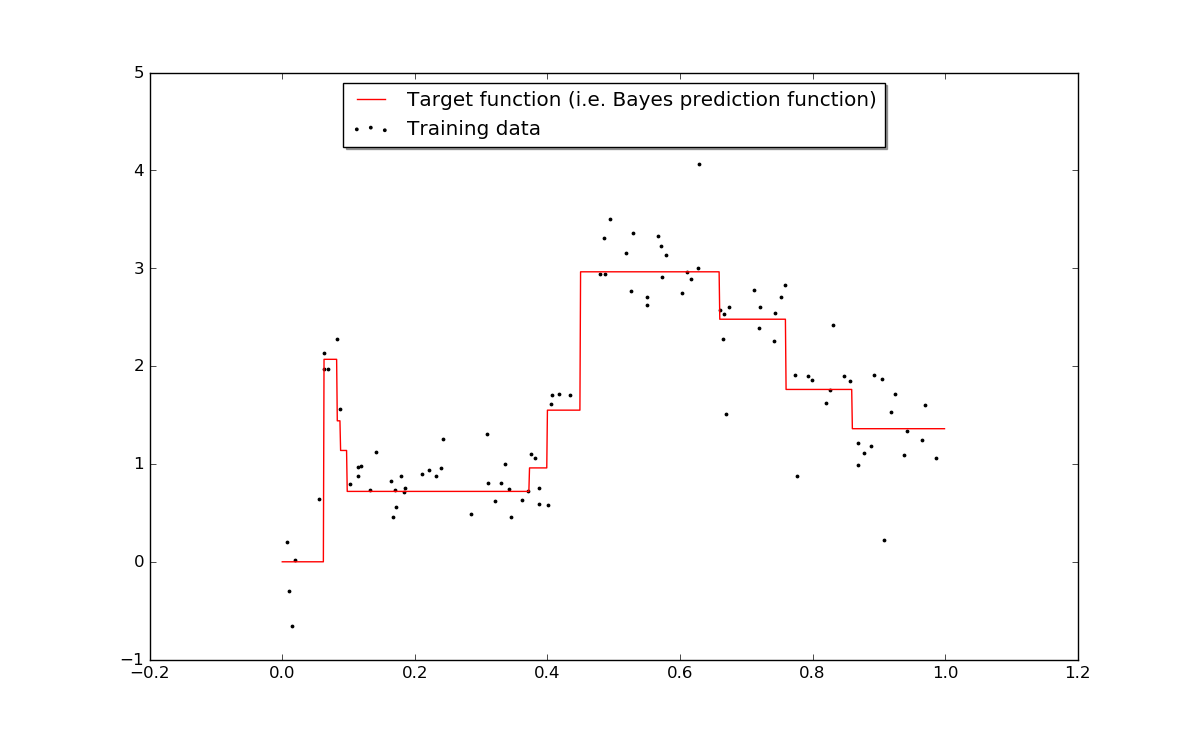
\includegraphics[height=2.5in]{figures/training-data-and-target-fn}
\par\end{centering}
\caption{\label{fig:Training-data-and-target-fn}Training data and target function
we will be considering in this assignment.}
\end{figure}

You can examine how the target function and the data were generated
by looking at \texttt{setup\_problem.py.} The figure can be reproduced
by running the \texttt{LOAD\_PROBLEM} branch of the main function. 

As you can see, the target function is a highly nonlinear function
of the input. To handle this sort of problem with linear hypothesis
spaces, we will need to create a set of features that perform nonlinear
transforms of the input. A detailed description of the technique we
will use can be found in the Jupyter notebook \texttt{basis-fns.ipynb},
included in the zip file. 

In this assignment, we are providing you with a function that takes
care of the featurization. This is the ``featurize'' function, returned
by the \texttt{generate\_problem} function in \texttt{setup\_problem.py}.
The \texttt{generate\_problem} function also gives the true target
function, which has been constructed to be a sparse linear combination
of our features. The coefficients of this linear combination are also
provided by \texttt{generate\_problem}, so you can compare the coefficients
of the linear functions you find to the target function coefficients\@.
The \texttt{generate\_problem} function also gives you the train and
validation sets that you should use\@.

To get familiar with using the data, and perhaps to learn some techniques,
it's recommended that you work through the main() function of the
include file ridge\_regression.py. You'll go through the following
steps (on your own - no need to submit):
\begin{enumerate}
\item Load the problem from disk into memory with load\_problem.
\item Use the featurize function to map from a one-dimensional input space
to a $d$-dimensional feature space.
\item Visualize the design matrix of the featurized data. (All entries are
binary, so we will not do any data normalization or standardization
in this problem, though you may experiment with that on your own.)
\item Take a look at the class \texttt{RidgeRegression}. Here we've implemented
our own \texttt{RidgeRegression} using the general purpose optimizer
provided by scipy.optimize. This is primarily to introduce you to
the sklearn framework, if you are not already familiar with it. It
can help with hyperparameter tuning, as we will see shortly.
\item Take a look at compare\_our\_ridge\_with\_sklearn. In this function,
we want to get some evidence that our implementation is correct, so
we compare to sklearn's ridge regression. Comparing the outputs of
two implementations is not always trivial \textendash{} often the
objective functions are slightly different, so you may need to think
a bit about how to compare the results. In this case, sklearn has
total square loss rather than average square loss, so we needed to
account for that. In this case, we get an almost exact match with
sklearn. This is because ridge regression is a rather easy objective
function to optimize. You may not get as exact a match for other objective
functions, even if both methods are ``correct.''
\item Next take a look at do\_grid\_search, in which we demonstrate how
to take advantage of the fact that we've wrapped our ridge regression
in an sklearn ``Estimator'' to do hyperparameter tuning. It's a
little tricky to get GridSearchCV to use the train/test split that
you want, but an approach is demonstrated in this function. In the
line assigning the param\_grid variable, you can see my attempts at
doing hyperparameter search on a different problem. Below you will
be modifying this (or using some other method, if you prefer) to find
the optimal L2 regularization parameter for the data provided.
\item Next is some code to plot the results of the hyperparameter search.
\item Next we want to visualize some prediction functions. We plotted the
target function, along with several prediction functions corresponding
to different regularization parameters, as functions of the original
input space $\reals$, along with the training data. Next we visualize
the coefficients of each feature with bar charts. Take note of the
scale of the $y$-axis, as they may vary substantially, buy default.
\end{enumerate}

\section{Ridge Regression}

In the problems below, you do not need to implement ridge regression.
You may use any of the code provided in the assignment, or you may
use other packages. However, your results must correspond to the ridge
regression objective function that we use, namely
\[
J(w;\lambda)=\frac{1}{n}\sum_{i=1}^{n}\left(w^{T}x_{i}-y_{i}\right)^{2}+\lambda\|w\|^{2}.
\]
\begin{enumerate}
\item Run ridge regression on the provided training dataset. Choose the
$\lambda$ that minimizes the empirical risk (i.e. the average square
loss) on the validation set. Include a table of the parameter values
you tried and the validation performance for each. Also include a
plot of the results.
\item Now we want to visualize the prediction functions. On the same axes,
plot the following: the training data, the target function, an unregularized
least squares fit (still using the featurized data), and the prediction
function chosen in the previous problem. Next, along the lines of
the bar charts produced by the code in compare\_parameter\_vectors,
visualize the coefficients for each of the prediction functions plotted,
including the target function. Describe the patterns, including the
scale of the coefficients, as well as which coefficients have the
most weight.
\item For the chosen $\lambda$, examine the model coefficients. For ridge
regression, we don't expect any parameters to be exactly $0$. However,
let's investigate whether we can predict the sparsity pattern of the
true parameters (i.e. which parameters are $0$ and which are nonzero)
by thresholding the parameter estimates we get from ridge regression.
We'll predict that $w_{i}=0$ if $\left|\hat{w}_{i}\right|<\eps$
and $w_{i}\neq0$ otherwise. Give the confusion matrix for $\eps=10^{-6},10^{-3},10^{-1}$,
and any other thresholds you would like to try.
\end{enumerate}

\section{\label{subsec:Shooting-algorithm}Coordinate Descent for Lasso (a.k.a.
The Shooting algorithm)}

The Lasso optimization problem can be formulated as\footnote{} 
\[
\hat{w}\in{\displaystyle \argmin_{w\in\reals^{d}}\sum_{i=1}^{m}(h_{w}(x_{i})-y_{i})^{2}+\lambda\|w\|_{1}},
\]
where $h_{w}(x)=w^{T}x$, and $\|w\|_{1}=\sum_{i=1}^{d}|w_{i}|$.
Note that to align with Murpy's formulation below, and for historical
reasons, we are using the total square loss, rather than the average
square loss, in the objective function.

Since the $\ell_{1}$-regularization term in the objective function
is non-differentiable, it's not immediately clear how gradient descent
or SGD could be used to solve this optimization problem directly.
(In fact, as we'll see in the next homework on SVMs, we can use ``subgradient''
methods when the objective function is not differentiable, in addition
to the two methods discussed in this homework assignment.)

Another approach to solving optimization problems is coordinate descent,
in which at each step we optimize over one component of the unknown
parameter vector, fixing all other components. The descent path so
obtained is a sequence of steps, each of which is parallel to a coordinate
axis in $\reals^{d}$, hence the name. It turns out that for the Lasso
optimization problem, we can find a closed form solution for optimization
over a single component fixing all other components. This gives us
the following algorithm, known as the \textbf{shooting algorithm}:
\begin{center}
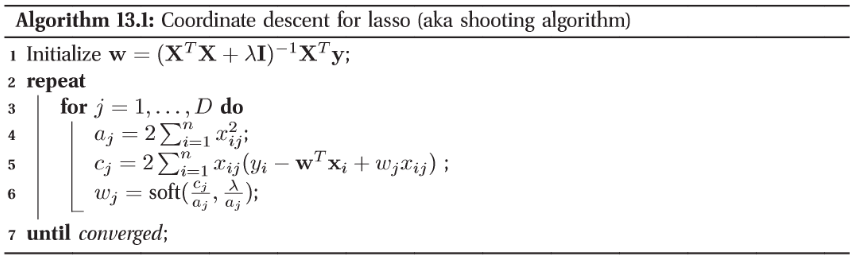
\includegraphics[width=1\textwidth]{figures/shooting_algo} (Source:
Murphy, Kevin P. Machine learning: a probabilistic perspective. MIT
press, 2012.) 
\par\end{center}

The ``soft thresholding'' function is defined as
\[
\text{soft}\left(a,\delta\right)=\text{sign}(a)\left(\left|a\right|-\delta\right)_{+},
\]
for any $a,\delta\in\reals$. 

NOTE: Algorithm 13.1 does not account for the case that $a_{j}=c_{j}=0$,
which occurs when the $j$th column of $X$ is  identically $0$.
One can either eliminate the column (as it cannot possibly help the
solution), or you can set $w_{j}=0$ in that case since it is, as
you can easily verify, the coordinate minimizer. Note also that Murphy
is suggesting to initialize the optimization with the ridge regession
solution. Although theoretically this is not necessary (with exact
computations and enough time, coordinate descent will converge for
lasso from any starting point), in practice it's helpful to start
as close to the solution as we're able.

There are a few tricks that can make selecting the hyperparameter
$\lambda$ easier and faster. First, as we'll see in a later problem,
you can show that for any $\lambda\ge2\|X^{T}(y-\bar{y})\|_{\infty}$,
the estimated weight vector $\hat{w}$ is entirely zero, where $\bar{y}$
is the mean of values in the vector $y$, and $\|\cdot\|_{\infty}$
is the infinity norm (or supremum norm), which is the maximum over
the absolute values of the components of a vector. Thus we need to
search for an optimal $\lambda$ in $\left[0,\lambda_{\text{max}}\right]$,
where $\lambda_{\text{max}}=2\|X^{T}(y-\bar{y})\|_{\infty}$. (Note:
This expression for $\lambda_{\text{max}}$ assumes we have an unregularized
bias term in our model. That is, our decision functions are of the
form $h_{w,b}(x)=w^{T}x+b$. In our the experiments, we do not have
an unregularized bias term, so we should use $\lambda_{\text{max}}=2\|X^{T}y\|_{\infty}$.)

The second trick is to use the fact that when $\lambda$ and $\lambda'$
are close, the corresponding solutions $\hat{w}(\lambda)$ and $\hat{w}(\lambda')$
are also close. Start with $\lambda=\lambda_{\text{max}}$, for which
we know $\hat{w}(\lambda_{\text{max}})=0$. You can run the optimization
anyway, and initialize the optimization at $w=0$. Next, $\lambda$
is reduced (e.g. by a constant factor close to $1$), and the optimization
problem is solved using the previous optimal point as the starting
point. This is called \textbf{warm starting} the optimization. The
technique of computing a set of solutions for a chain of nearby $\lambda$'s
is called a \textbf{continuation }or\textbf{ homotopy method}. The
resulting set of parameter values $\hat{w}(\lambda)$ as $\lambda$
ranges over $\left[0,\lambda_{\text{max }}\right]$ is known as a
\textbf{regularization path}.

\subsection{Experiments with the Shooting Algorithm}
\begin{enumerate}
\item \label{enu:vectorization}The algorithm as described above is not
ready for a large dataset (at least if it has being implemented in
Python) because of the implied loop in the summation signs for the
expressions for $a_{j}$ and $c_{j}$. Give an expression for computing
$a_{j}$ and $c_{j}$ using matrix and vector operations, without
explicit loops. This is called ``vectorization'' and can lead to
dramatic speedup when implemented in languages such as Python, Matlab,
and R. Write your expressions using $X$, $w$, $y=\left(y_{1},\ldots,y_{n}\right)^{T}$
(the column vector of responses), $X_{\cdot j}$ (the $j$th column
of $X$, represented as a column matrix), and $w_{j}$ (the $j$th
coordinate of $w$ \textendash{} a scalar).\\
\item \begin{flushleft}
Write a function that computes the Lasso solution for a given $\lambda$
using the shooting algorithm described above. For convergence criteria,
continue coordinate descent until a pass through the coordinates reduces
the objective function by less than $10^{-8}$, or you have taken
1000 passes through the coordinates. Compare performance of cyclic
coordinate descent to randomized coordinate descent, where in each
round we pass through the coordinates in a different random order
(for your choices of $\lambda$). Compare also the solutions attained
(following the convergence criteria above) for starting at $0$ versus
starting at the ridge regression solution suggested by Murphy (again,
for your choices of $\lambda$). If you like, you may adjust the convergence
criteria to try to attain better results (or the same results faster).
\par\end{flushleft}
\item \begin{flushleft}
Run your best Lasso configuration on the training dataset provided,
and select the $\lambda$ that minimizes the square error on the validation
set. Include a table of the parameter values you tried and the validation
performance for each. Also include a plot of these results. Include
also a plot of the prediction functions, just as in the ridge regression
section, but this time add the best performing Lasso prediction function
and remove the unregularized least squares fit. Similarly, add the
lasso coefficients to the bar charts of coefficients generated in
the ridge regression setting. Comment on the results, with particular
attention to parameter sparsity and how the ridge and lasso solutions
compare. What's the best model you found, and what's its validation
performance?\\
\par\end{flushleft}

\item \label{enu:homotopy}Implement the homotopy method described above.
Compute the Lasso solution for (at least) the regularization parameters
in the set $\left\{ \lambda=\lambda_{\text{max}}0.8^{i}\mid i=0,\ldots,29\right\} $.
Plot the results (average validation loss vs $\lambda$).
\item {[}Optional{]} Note that the data in Figure \ref{fig:Training-data-and-target-fn}
is almost entirely nonnegative. Since we don't have an unregularized
bias term, we have ``pay for'' this offset using our penalized parameters.
Note also that $\lambda_{\text{max}}$ would decrease significantly
if the $y$ values were $0$ centered (using the training data, of
course), or if we included an unregularized bias term. Experiment
with one or both of these approaches, for both and lasso and ridge
regression, and report your findings.
\end{enumerate}

\subsection{{[}Optional{]} Deriving the Coordinate Minimizer for Lasso}

This problem is to derive the expressions for the coordinate minimizers
used in the Shooting algorithm. This is often \href{http://davidrosenberg.github.io/mlcourse/Archive/2015/Lectures/2.Lab.subgradient-descent.pdf\#page=15}{derived using subgradients (slide 15)},
but here we will take a bare hands approach (which is essentially
equivalent). 

In each step of the shooting algorithm, we would like to find the
$w_{j}$ minimizing
\begin{eqnarray*}
f(w_{j}) & = & \sum_{i=1}^{n}\left(w^{T}x_{i}-y_{i}\right)^{2}+\lambda\left|w\right|_{1}\\
 & = & \sum_{i=1}^{n}\left[w_{j}x_{ij}+\sum_{k\neq j}w_{k}x_{ik}-y_{i}\right]^{2}+\lambda\left|w_{j}\right|+\lambda\sum_{k\neq j}\left|w_{k}\right|,
\end{eqnarray*}
where we've written $x_{ij}$ for the $j$th entry of the vector $x_{i}$.
This function is convex in $w_{j}$. The only thing keeping $f$ from
being differentiable is the term with $\left|w_{j}\right|$. So $f$
is differentiable everywhere except $w_{j}=0$. We'll break this problem
into 3 cases: $w_{j}>0$, $w_{j}<0$, and $w_{j}=0$. In the first
two cases, we can simply differentiate $f$ w.r.t. $w_{j}$ to get
optimality conditions. For the last case, we'll use the fact that
since $f:\reals\to\reals$ is convex, 0 is a minimizer of $f$ iff
\[
\lim_{\eps\downarrow0}\frac{f(\eps)-f(0)}{\eps}\ge0\quad\mbox{and}\quad\lim_{\eps\downarrow0}\frac{f(-\eps)-f(0)}{\eps}\ge0.
\]
This is a special case of the optimality conditions described in \href{https://github.com/davidrosenberg/mlcourse/blob/gh-pages/Archive/2017/Lectures/2.Lab.directional-derivatives.pdf\#page=6}{slide 6 here},
where now the ``direction'' $v$ is simply taken to be the scalars
$1$ and $-1$, respectively. 
\begin{enumerate}
\item First let's get a trivial case out of the way. If $x_{ij}=0$ for
$i=1,\ldots,n$, what is the coordinate minimizer $w_{j}$? In the
remaining questions below, you may assume that $\sum_{i=1}^{n}x_{ij}^{2}>0$.
\item Give an expression for the derivative $f(w_{j})$ for $w_{j}\neq0$.
It will be convenient to write your expression in terms of the following
definitions:
\begin{eqnarray*}
\sign(w_{j}) & := & \begin{cases}
1 & w_{j}>0\\
0 & w_{j}=0\\
-1 & w_{j}<0
\end{cases}\\
a_{j} & := & 2\sum_{i=1}^{n}x_{ij}^{2}\\
c_{j} & := & 2\sum_{i=1}^{n}x_{ij}\left(y_{i}-\sum_{k\neq j}w_{k}x_{ik}\right).
\end{eqnarray*}
\item If $w_{j}>0$ and minimizes $f$, show that $w_{j}=\frac{1}{a_{j}}\left(c_{j}-\lambda\right)$.
Similarly, if $w_{j}<0$ and minimizes $f$, show that $w_{j}=\frac{1}{a_{j}}\left(c_{j}+\lambda\right)$.
Give conditions on $c_{j}$ that imply that a minimizer $w_{j}$ is
positive and conditions for which a minimizer $w_{j}$ is negative.
\item Derive expressions for the two one-sided derivatives at $f(0)$, and
show that $c_{j}\in\left[-\lambda,\lambda\right]$ implies that $w_{j}=0$
is a minimizer.
\item Putting together the preceding results, we conclude the following:
\[
w_{j}=\begin{cases}
\frac{1}{a_{j}}\left(c_{j}-\lambda\right) & c_{j}>\lambda\\
0 & c_{j}\in[-\lambda,\lambda]\\
\frac{1}{a_{j}}\left(c_{j}+\lambda\right) & c_{j}<-\lambda
\end{cases}
\]
Show that this is equivalent to the expression given in \ref{subsec:Shooting-algorithm}.
\end{enumerate}

\section{Lasso Properties}

\subsection{Deriving $\lambda_{\mbox{max}}$}

In this problem we will derive an expression for $\lambda_{\text{max}}$.
For the first three parts, use the Lasso objective function excluding
the bias term i.e, $J(w)=\left\Vert Xw-y\right\Vert _{2}^{2}+\lambda\left\Vert w\right\Vert _{1}$.
We will show that for any $\lambda\geq2\|X^{T}y\|_{\infty}$, the
estimated weight vector $\hat{w}$ is entirely zero, where $\|\cdot\|_{\infty}$
is the infinity norm (or supremum norm), which is the maximum absolute
value of any component of the vector. 
\begin{enumerate}
\item The one-sided directional derivative of $f(x)$ at $x$ in the direction
$v$ is defined as:
\[
f'(x;v)=\lim_{h\downarrow0}\frac{f(x+hv)-f(x)}{h}
\]
Compute $J'(0;v)$. That is, compute the one-sided directional derivative
of $J(w)$ at $w=0$ in the direction $v$. {[}Hint: the result should
be in terms of $X,y,\lambda,\text{ and }v$.{]}
\item Since the Lasso objective is convex, $w^{*}$ is a minimizer of $J(w)$
if and only if the directional derivative $J'(w^{*};v)\geq0$ for
all $v\neq0$. Show that for any $v\neq0$, we have $J'(0;v)\ge0$
if and only if $\lambda\ge C$, for some $C$ that depends on $X,y,\text{ and }v$.
You should have an explicit expression for $C$.  \textbf{}\\
\textbf{}\\
\item In the previous problem, we get a different lower bound on $\lambda$
for each choice of $v$. Show that the maximum of these lower bounds
on $\lambda$ is $\lambda_{\text{max}}=2\|X^{T}y\|_{\infty}$. Conclude
that $w=0$ is a minimizer of $J(w)$ if and only if $\lambda\ge2\|X^{T}y\|_{\infty}$.
\\
\item {[}Optional{]} Let $J(w,b)=\left\Vert Xw+b\mathbf{1}-y\right\Vert _{2}^{2}+\lambda\left\Vert w\right\Vert _{1}$,
where $\mathbf{1}\in\reals^{n}$ is a column vector of $1$'s. Let
$\bar{y}$ be the mean of values in the vector $y$. Show that $(w^{*},b^{*})=(0,\bar{y})$
is a minimizer of $J(w,b)$ if and only if $\lambda\ge\lambda_{\text{max}}=2\|X^{T}(y-\bar{y})\|_{\infty}$.\\
\end{enumerate}

\subsection{Feature Correlation}

In this problem, we will examine and compare the behavior of the Lasso
and ridge regression in the case of an exactly repeated feature. That
is, consider the design matrix $X\in\reals^{m\times d}$, where $X_{\cdot i}=X_{\cdot j}$
for some $i$ and $j$, where $X_{\cdot i}$ is the $i^{th}$ column
of $X$. We will see that ridge regression divides the weight equally
among identical features, while Lasso divides the weight arbitrarily.
In an optional part to this problem, we will consider what changes
when $X_{\cdot i}$ and $X_{\cdot j}$ are highly correlated (e.g.
exactly the same except for some small random noise) rather than exactly
the same. 
\begin{enumerate}
\item Without loss of generality, assume the first two colums of $X$ are
our repeated features. Partition $X$ and $\theta$ as follows:\\
\[
X=\left(\begin{array}{ccc}
x_{1} & x_{2} & X_{r}\end{array}\right)\qquad\theta=\left(\begin{array}{c}
\theta_{1}\\
\theta_{2}\\
\theta_{r}
\end{array}\right)
\]
We can write the Lasso objective function as:
\begin{align*}
J(\theta)= & \left\Vert X\theta-y\right\Vert _{2}^{2}+\lambda\left\Vert \theta\right\Vert _{1}\\
= & \left\Vert x_{1}\theta_{1}+x_{2}\theta_{2}+X_{r}\theta_{r}-y\right\Vert _{2}^{2}+\lambda\vert\theta_{1}\vert+\lambda\vert\theta_{2}\vert+\lambda\left\Vert \theta_{r}\right\Vert _{1}
\end{align*}
With repeated features, there will be multiple minimizers of $J(\theta)$.
Suppose that 
\[
\hat{\theta}=\begin{pmatrix}a\\
b\\
r
\end{pmatrix}
\]
is a minimizer of $J(\theta)$. Give conditions on $c$ and $d$ such
that $\left(c,d,r^{T}\right)^{T}$ is also a minimizer of $J(\theta$).
{[}Hint: First show that $a$ and $b$ must have the same sign, or
at least one of them is zero. Then, using this result, rewrite the
optimization problem to derive a relation between $a$ and $b$.{]}\\
\item Using the same notation as the previous problem, suppose 
\[
\hat{\theta}=\begin{pmatrix}a\\
b\\
r
\end{pmatrix}
\]
minimizes the ridge regression objective function. What is the relationship
between $a$ and $b$, and why? \\
\item {[}Optional{]} What do you think would happen with Lasso and ridge
when $X_{\cdot i}$ and $X_{\cdot j}$ are highly correlated, but
not exactly the same. You may investigate this experimentally or theoretically.
\end{enumerate}

\section{{[}Optional{]} The Ellipsoids in the $\ell_{1}/\ell_{2}$ regularization
picture}

Recall the famous picture purporting to explain why $\ell_{1}$ regularization
leads to sparsity, while $\ell_{2}$ regularization does not. Here's
the instance from Hastie et al's \emph{The Elements of Statistical
Learning:}
\begin{center}
\includegraphics[width=0.5\paperwidth]{figures/L1-L2-corner-pic-ESL-Fig3\lyxdot 11} 
\par\end{center}

(While Hastie et al. use $\beta$ for the parameters, we'll continue
to use $w$.) 

In this problem we'll show that the level sets of the empirical risk
are indeed ellipsoids centered at the empirical risk minimizer $\hat{w}$.

Consider linear prediction functions of the form $x\mapsto w^{T}x$.
Then the empirical risk for $f(x)=w^{T}x$ under the square loss is
\begin{eqnarray*}
\hat{R}_{n}(w) & = & \frac{1}{n}\sum_{i=1}^{n}\left(w^{T}x_{i}-y_{i}\right)^{2}\\
 & = & \frac{1}{n}\left(Xw-y\right)^{T}\left(Xw-y\right).
\end{eqnarray*}
\begin{enumerate}
\item {[}Optional{]} Let $\hat{w}=\left(X^{T}X\right)^{-1}X^{T}y$. Show
that $\hat{w}$ has empirical risk given by 
\[
\hat{R}_{n}(\hat{w})=\frac{1}{n}\left(-y^{T}X\hat{w}+y^{T}y\right)
\]
\\
\item {[}Optional{]} \label{enu:emprisk-ellipsoid}Show that for any $w$
we have
\[
\hat{R}_{n}(w)=\frac{1}{n}\left(w-\hat{w}\right)^{T}X^{T}X\left(w-\hat{w}\right)+\hat{R}_{n}(\hat{w}).
\]
Note that the RHS (i.e. ``right hand side'') has one term that's
quadratic in $w$ and one term that's independent of $w$. In particular,
the RHS does not have any term that's linear in $w$. On the LHS (i.e.
``left hand side''), we have $\hat{R}_{n}(w)=\frac{1}{n}\left(Xw-y\right)^{T}\left(Xw-y\right)$.
After expanding this out, you'll have terms that are quadratic, linear,
and constant in $w$. Completing the square is the tool for rearranging
an expression to get rid of the linear terms. The following ``completing
the square'' identity is easy to verify just by multiplying out the
expressions on the RHS:
\begin{eqnarray*}
x^{T}Mx-2b^{T}x & = & \left(x-M^{-1}b\right)^{T}M(x-M^{-1}b)-b^{T}M^{-1}b
\end{eqnarray*}
\\
\item {[}Optional{]} Using the expression derived for $\hat{R}_{n}(w)$
in \ref{enu:emprisk-ellipsoid}, give a very short proof that $\hat{w}=\left(X^{T}X\right)^{-1}X^{T}y$
is the empirical risk minimizer. That is: 
\[
\hat{w}=\argmin_{w}\hat{R}_{n}(w).
\]
Hint: Note that $X^{T}X$ is positive semidefinite and, by definition,
a symmetric matrix $M$ is positive semidefinite iff for all $x\in\reals^{d}$,
$x^{T}Mx\ge0$.\\
 
\item {[}Optional{]} Give an expression for the set of $w$ for which the
empirical risk exceeds the minimum empirical risk $\hat{R}_{n}(\hat{w})$
by an amount $c>0$. If $X$ is full rank, then $X^{T}X$ is positive
definite, and this set is an ellipse \textendash{} what is its center?\\
\end{enumerate}

\section{{[}Optional{]} Projected SGD via Variable Splitting}

In this question, we consider another general technique that can be
used on the Lasso problem. We first use the variable splitting method
to transform the Lasso problem to a differentiable problem with linear
inequality constraints, and then we can apply a variant of SGD.

Representing the unknown vector $\theta$ as a difference of two non-negative
vectors $\theta^{+}$ and $\theta^{-}$, the $\ell{}_{1}$-norm of
$\theta$ is given by ${\displaystyle \sum_{i=1}^{d}\theta_{i}^{+}}$
+ ${\displaystyle \sum_{i=1}^{d}\theta_{i}^{-}}$. Thus, the optimization
problem can be written as 
\begin{gather*}
(\hat{\theta}^{+},\hat{\theta}^{-})={\displaystyle \argmin_{\theta^{+},\theta^{-}\in\reals^{d}}\sum_{i=1}^{m}(h_{\theta^{+},\theta^{-}}(x_{i})-y_{i})^{2}+\lambda\sum_{i=1}^{d}\theta_{i}^{+}+\lambda\sum_{i=1}^{d}\theta_{i}^{-}}\\
\mbox{such that }\theta^{+}\ge0\mbox{ and }\theta^{-}\ge0,
\end{gather*}
where $h_{\theta^{+},\theta^{-}}(x)=(\theta^{+}-\theta^{-})^{T}x$.
The original parameter $\theta$ can then be estimated as $\hat{\theta}=(\hat{\theta}^{+}-\hat{\theta}^{-})$.

This is a convex optimization problem with a differentiable objective
and linear inequality constraints. We can approach this problem using
projected stochastic gradient descent, as discussed in lecture. Here,
after taking our stochastic gradient step, we project the result back
into the feasible set by setting any negative components of $\theta^{+}$
and $\theta^{-}$ to zero.
\begin{enumerate}
\item {[}Optional{]} Implement projected SGD to solve the above optimization
problem for the same $\lambda$'s as used with the shooting algorithm.
Since the two optimization algorithms should find essentially the
same solutions, you can check the algorithms against each other. Report
the differences in validation loss for each $\lambda$ between the
two optimization methods. (You can make a table or plot the differences.)
\\
\item {[}Optional{]} Choose the $\lambda$ that gives the best performance
on the validation set. Describe the solution $\hat{w}$ in term of
its sparsity. How does the sparsity compare to the solution from the
shooting algorithm?\\
 
\end{enumerate}

\end{document}
